\documentclass[a4paper, 12pt]{article}
\usepackage{geometry}
\geometry{a4paper,
total={170mm,257mm},left=2cm,right=2cm,
top=2cm,bottom=2cm}

\usepackage{mathtext}
\usepackage{amsmath}
\usepackage[utf8]{inputenc}
\usepackage[english,russian]{babel}
\usepackage{graphicx}
\usepackage{float}
\usepackage{tabularx, colortbl}
\usepackage{caption}
\usepackage{textcomp}
\usepackage{multirow}

\captionsetup{labelsep=period}

\newcommand{\parag}[1]{\paragraph*{#1:}}
\DeclareSymbolFont{T2Aletters}{T2A}{cmr}{m}{it}

\newcounter{Points}
\setcounter{Points}{1}
\newcommand{\point}{\arabic{Points}. \addtocounter{Points}{1}}

\newcolumntype{C}{>{\centering\arraybackslash}X}
\renewcommand\labelenumi{\theenumi)}

\author{Калинин Данил, Б01-110}
\date{07.09.2021}
\title{Лабораторная работа 1.1.4.\\Измерение интенсивности радиационного фона}

\begin{document}
\maketitle

\parag {Цель работы}
применение методов обработки экспериментальных данных для изучения статистических закономерностей при измерении интенсивности радиационного фона

\parag {В работе используются}
счетчик Гейгера-Мюллера (СТС-6), блок питания, компьютер с интерфейсом связи со счетчиком.

\parag {Теоритическая справка} ~\\
Среднеквадратичная ошибка числа отчетов, измеренного за некоторый интервал времени равна:

\begin{equation} \label{eq:1}
    \sigma = \sqrt{n}
\end{equation}

Тогда результат измерения запишется так:

\begin{equation} \label{eq:2}
    n_0 = n \pm \sqrt{n}
\end{equation}

При $N$ измеренях среднее значение числа посчитанных за одно измрение частиц может быть посчитано по форумле:

\begin{equation} \label{eq:3}
    \bar{n} = \frac{1}{N} \sum_{i=1}^N {n_i}
\end{equation}

А стандартная ошибка отдельного измерения может быть оценена по формуле:

\begin{equation} \label{eq:4}
    \sigma_{отд} = \sqrt {\frac{1}{N} \sum_{i=1}^N ({n_i - \bar{n}})^2}
\end{equation}

В соответствии с формулой \eqref{eq:1} следует ожидать, что это ошибка будет близка к $\sqrt{n_i}$.  Поскольку $n_i$ различны, мы будем получать различные оценки для $\sigma_{отд}$. Какие-то из них будут лучше, какие-то -- хуже. Ближе всего к значению $\sigma_{отд}$ будет корень из усредненного измерения, т.е.

\begin{equation} \label{eq:5}
    \sigma_{отд} \approx \sqrt{\bar{n}}
\end{equation}

Величина $\bar{n}$ из формулы \eqref{eq:3} тоже является случайной, ее отклонене от истинного значения может быть определено по формуле:

\begin{equation} \label{eq:6}
    \sigma_{\bar{n}} = \frac{1}{N} \sqrt {\sum_{i=1}^N ({n_i - \bar{n}})^2} = \frac {\sigma_{отд}}{\sqrt {N}}
\end{equation}

Обычно наибольший интерес представляет относительная погрешность. Для рассмотрения серии из $N$ экспериментов по 20 с. относительная ошибка отдельного измерения (т.е. ожидаемое отличие $n_i$ от $n_0$) равна:

\begin{equation} \label{eq:7}
   \varepsilon_{отд} = \frac {\sigma_{отд}}{n_i} \approx \frac {1}{\sqrt {n_i}}
\end{equation}

Аналогичным образом определяется относительная ошибка в опредлении среднего по всем измерениям значения $\bar{n}$.

\begin{equation} \label{eq:8}
    \varepsilon_{\bar{n}} = \frac {\sigma_{\bar{n}}}{\bar{n}} = \frac {\sigma_{отд}}{\bar{n} \sqrt {N}} \approx \frac {1}{\sqrt {\bar {n} N}}
\end{equation}

\parag {Ход работы} ~\\

\point Включим компьютер и проведем демонстрационный эксперимент, чтобы познакомится с интерфейсом программы. Заметим, что:
\begin{enumerate}
    \item измеряемая величина флуктуирует;
    \item флуктуации среднего значения измеряемой величины уменьшаются и среднее значение величины выходит на постоянный уровень;
    \item флуктуации величины погрешности отдельного измерения уменьшаются, и погрешность отдельного измерения (погрешность метода) выходит на постоянную величину;
    \item флуктуации величины погрешности среднего значения уменьшаются, а сама величина убывает.   
\end{enumerate}


\point Переходим к основному эксперименту: измерение плотности потока космического излучения за 20 с. На компьютере проведем обработку, аналогичную сделанной в демонстрационном эксперименте. Результаты приведем в таблицы \ref{tabl:data_raw_20} и \ref{tabl:data_hist_10}. Примечание: таблица \ref{tabl:data_raw_20} устроена так, что, например, результат 123-го опыта лежит на пересечении строки, обозначенной 120 и столбца с номером 3.

\begin{table}[!h]
    \centering
    \begin{tabularx}{\textwidth}
        {|C|C|C|C|C|C|C|C|C|C|C|}
        \hline
        \textbf{\textnumero \quad опыта} & \textbf{1 } & \textbf{2 } & \textbf{3 } & \textbf{4 } & \textbf{5 } & \textbf{6 } & \textbf{7 } & \textbf{8 } & \textbf{9 } & \textbf{10}  \\ \hline
        \textbf{0}   & 31 & 43 & 22 & 21 & 22 & 31 & 33 & 30 & 21 & 25 \\ \hline
        \textbf{10 } & 26 & 34 & 26 & 29 & 32 & 32 & 30 & 28 & 28 & 28 \\ \hline
        \textbf{20 } & 20 & 26 & 16 & 25 & 29 & 34 & 29 & 30 & 31 & 26 \\ \hline
        \textbf{30 } & 28 & 38 & 30 & 20 & 22 & 24 & 29 & 30 & 20 & 21 \\ \hline
        \textbf{40 } & 27 & 24 & 37 & 25 & 31 & 34 & 37 & 23 & 23 & 28 \\ \hline
        \textbf{50 } & 25 & 32 & 38 & 21 & 33 & 41 & 25 & 31 & 21 & 30 \\ \hline
        \textbf{60 } & 18 & 29 & 24 & 38 & 19 & 37 & 30 & 26 & 25 & 42 \\ \hline
        \textbf{70 } & 23 & 23 & 30 & 22 & 25 & 28 & 25 & 26 & 18 & 36 \\ \hline
        \textbf{80 } & 26 & 20 & 25 & 32 & 22 & 41 & 34 & 23 & 26 & 22 \\ \hline
        \textbf{90 } & 30 & 27 & 26 & 34 & 26 & 34 & 36 & 15 & 23 & 29 \\ \hline
        \textbf{100} & 27 & 29 & 15 & 24 & 29 & 36 & 34 & 35 & 27 & 31 \\ \hline
        \textbf{110} & 26 & 42 & 24 & 36 & 26 & 29 & 30 & 23 & 28 & 30 \\ \hline
        \textbf{120} & 36 & 26 & 27 & 30 & 24 & 28 & 24 & 20 & 30 & 25 \\ \hline
        \textbf{130} & 24 & 29 & 26 & 13 & 21 & 19 & 23 & 34 & 26 & 28 \\ \hline
        \textbf{140} & 25 & 25 & 24 & 34 & 28 & 25 & 29 & 27 & 29 & 30 \\ \hline
        \textbf{150} & 24 & 33 & 33 & 26 & 33 & 16 & 35 & 25 & 28 & 29 \\ \hline
        \textbf{160} & 30 & 21 & 18 & 31 & 19 & 37 & 27 & 20 & 22 & 32 \\ \hline
        \textbf{170} & 31 & 34 & 28 & 17 & 24 & 35 & 20 & 33 & 20 & 19 \\ \hline
        \textbf{180} & 28 & 25 & 31 & 40 & 24 & 29 & 24 & 24 & 28 & 32 \\ \hline
        \textbf{190} & 27 & 34 & 27 & 35 & 26 & 29 & 16 & 28 & 31 & 29 \\ \hline
    \end{tabularx}
    \caption{Число срабатываний счетчика за 20 с.}
    \label{tabl:data_raw_20}
\end{table}

\begin{table}[!h]
    \centering
    \begin{tabularx}{\textwidth}
        {|C|C|C|}
        \hline
        \textbf{Число импульсов} & \textbf{Число случаев} & \textbf{Доля случаев} \\ \hline
        3  & 1  & 0.0025    \\ \hline
        4  & 1  & 0.0025    \\ \hline
        5  & 2  & 0.005     \\ \hline
        6  & 2  & 0.005     \\ \hline
        7  & 7  & 0.0175    \\ \hline
        8  & 14 & 0.035     \\ \hline
        9  & 19 & 0.0475    \\ \hline
        10 & 32 & 0.08      \\ \hline
        11 & 38 & 0.095     \\ \hline
        12 & 34 & 0.085     \\ \hline
        13 & 39 & 0.0975    \\ \hline
        14 & 39 & 0.0975    \\ \hline
        15 & 46 & 0.115     \\ \hline
        16 & 39 & 0.0975    \\ \hline
        17 & 24 & 0.06      \\ \hline
        18 & 21 & 0.0525    \\ \hline
        19 & 17 & 0.0425    \\ \hline
        20 & 11 & 0.00275   \\ \hline
        21 & 5  & 0.0125    \\ \hline
        22 & 4  & 0.01      \\ \hline
        23 & 3  & 0.0075    \\ \hline
        25 & 1  & 0.0025    \\ \hline
        28 & 1  & 0.0025    \\ \hline
    \end{tabularx}
    \caption{Данные для построения гистограммы распределения числа срабатываний счетчика за 10 с.}
    \label{tabl:data_hist_10}
\end{table}

\point Разобьем результаты из таблицы \ref{tabl:data_raw_20} в порядке их получения на группы по 2 и сложим числа в каждой группе. Это будет соответствовать $N_2=100$ измерениям по $t=40~c.$ каждое. Резльтаты сведем в таблицу \ref{tabl:data_raw_40}

\begin{table}[!h]
    \centering
    \begin{tabularx}{\textwidth}
        {|C|C|C|C|C|C|C|C|C|C|C|}
        \hline
        \textbf{\textnumero \quad опыта} & \textbf{1 } & \textbf{2 } & \textbf{3 } & \textbf{4 } & \textbf{5 } & \textbf{6 } & \textbf{7 } & \textbf{8 } & \textbf{9 } & \textbf{10}  \\ \hline
        \textbf{0} & 74 & 43 & 53 & 63 & 46 & 60 & 55 & 64 & 58 & 56 \\ \hline
        \textbf{10} & 46 & 41 & 63 & 59 & 57 & 66 & 50 & 46 & 59 & 41 \\ \hline
        \textbf{20} & 51 & 62 & 65 & 60 & 51 & 57 & 59 & 74 & 56 & 51 \\ \hline
        \textbf{30} & 47 & 62 & 56 & 56 & 67 & 46 & 52 & 53 & 51 & 54 \\ \hline
        \textbf{40} & 46 & 57 & 63 & 57 & 48 & 57 & 60 & 60 & 51 & 52 \\ \hline
        \textbf{50} & 56 & 39 & 65 & 69 & 58 & 68 & 60 & 55 & 53 & 58 \\ \hline
        \textbf{60} & 62 & 57 & 52 & 44 & 55 & 53 & 39 & 40 & 57 & 54 \\ \hline
        \textbf{70} & 50 & 58 & 53 & 56 & 59 & 57 & 59 & 49 & 60 & 57 \\ \hline
        \textbf{80} & 51 & 49 & 56 & 47 & 54 & 65 & 45 & 59 & 53 & 39 \\ \hline
        \textbf{90} & 53 & 71 & 53 & 48 & 60 & 61 & 62 & 55 & 44 & 60 \\ \hline
    \end{tabularx}
    \caption{Число срабатываний счетчика за 40 с.}
    \label{tabl:data_raw_40}
\end{table}

\point Представим результаты из таблицы \ref{tabl:data_raw_40} в виде, удобном для построения гистограммы. Результаты занесем в таблицу \ref{tabl:data_hist_40}. Гистограммы распределений среднего числа отсчетов за 10 и 40 с. строим на одном графике (рис \ref{pic:hists}). При этом для второй гистограммы увеличиваем шкалу деления оси абсцисс в 4 раза, чтобы максимумы гистограмм совпали.

\begin{table}[!h]
    \centering
    \begin{tabularx}{\textwidth}
        {|C|C|C|}
        \hline
        \textbf{Число импульсов} & \textbf{Число случаев} & \textbf{Доля случаев} \\ \hline
        39 & 3 & 0.03 \\ \hline
        40 & 1 & 0.01 \\ \hline
        41 & 2 & 0.02 \\ \hline
        43 & 1 & 0.01 \\ \hline
        44 & 2 & 0.02 \\ \hline
        45 & 1 & 0.01 \\ \hline
        46 & 5 & 0.05 \\ \hline
        47 & 2 & 0.02 \\ \hline
        48 & 2 & 0.02 \\ \hline
        49 & 2 & 0.02 \\ \hline
        50 & 2 & 0.02 \\ \hline
        51 & 6 & 0.06 \\ \hline
        52 & 3 & 0.03 \\ \hline
        53 & 8 & 0.08 \\ \hline
        54 & 3 & 0.03 \\ \hline
        55 & 4 & 0.04 \\ \hline
        56 & 7 & 0.07 \\ \hline
        57 & 9 & 0.09 \\ \hline
        58 & 4 & 0.04 \\ \hline
        59 & 6 & 0.06 \\ \hline
        60 & 8 & 0.08 \\ \hline
        61 & 1 & 0.01 \\ \hline
        62 & 4 & 0.04 \\ \hline
        63 & 3 & 0.03 \\ \hline
        64 & 1 & 0.01 \\ \hline
        65 & 3 & 0.03 \\ \hline
        66 & 1 & 0.01 \\ \hline
        67 & 1 & 0.01 \\ \hline
        68 & 1 & 0.01 \\ \hline
        69 & 1 & 0.01 \\ \hline
        71 & 1 & 0.01 \\ \hline
        74 & 2 & 0.02 \\ \hline
    \end{tabularx}
    \caption{Данные для построения гистограммы распределения числа срабатываний счетчика за 40 с.}
    \label{tabl:data_hist_40}
\end{table}

\begin{figure}[h!]
    \centering
    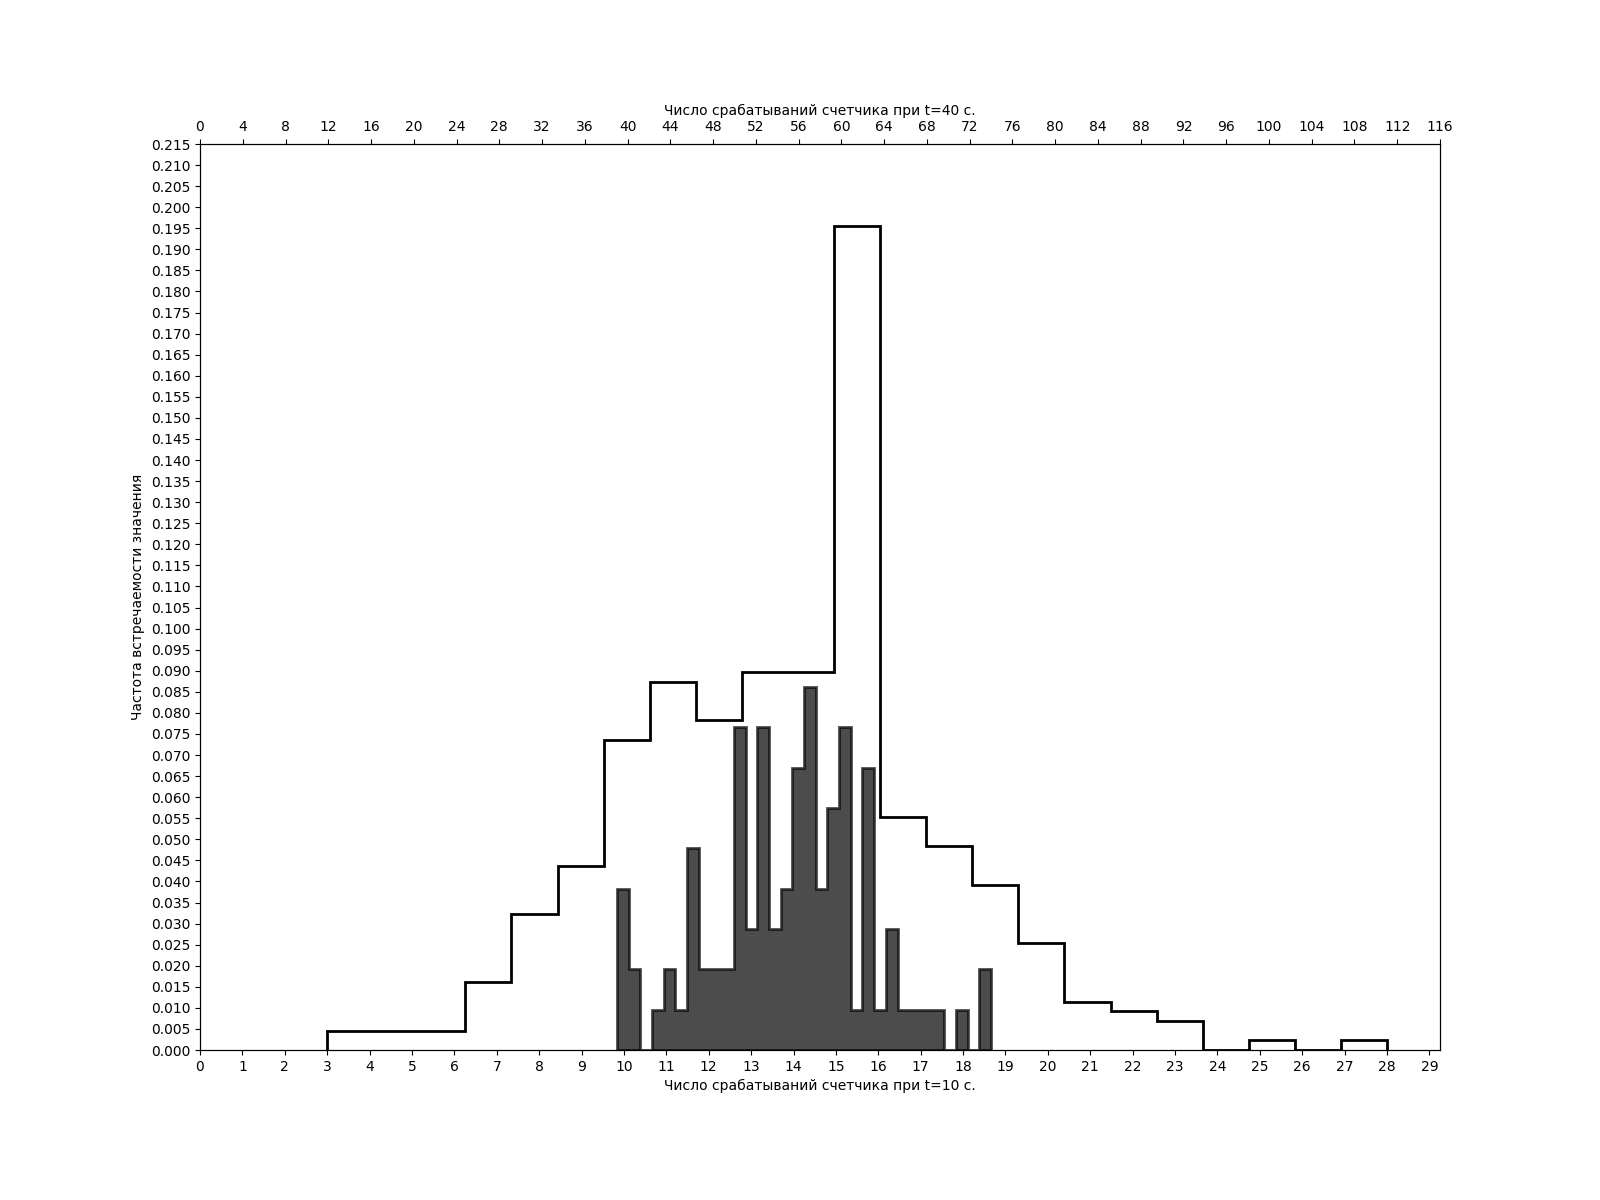
\includegraphics[width=\textwidth]{hists_plot.png}
    \caption{Гистограммы для $\tau=10~c.$ и $\tau=40~c.$}
    \label{pic:hists}
\end{figure}  

\point Используя формулу \ref{eq:3}, определим среднее значение срабатывания счетчика за 10  и 40 с. соответственно:
\[
    \bar{n}_{10} = \frac{1}{N_1} \sum_{i=1}^{N_{1}} {n_i} = \frac{5518}{400} = 13.795
\]

\[
    \bar{n}_{40} = \frac{1}{N_2} \sum_{i=1}^{N_{2}} {n_i} = \frac{5518}{100} = 55.18
\]

\point Найдем среднеквадратичную ошибку отдельного измерения по формуле \eqref{eq:4}
\[
    \sigma_{отд_{10}} = \sqrt {\frac{1}{N_1} \sum_{i=1}^{N_{1}} ({n_i - \bar{n}})^2} = 3.70175
\]

\[
    \sigma_{отд_{40}} = \sqrt {\frac{1}{N_2} \sum_{i=1}^{N_{2}} ({n_i - \bar{n}})^2} = 7.46107
\]

\point Убедимся в верности формулы \eqref{eq:5}. Действительно:
\[
    \sigma_{отд_{10}} = 3.70175 \approx \sqrt{13.795} = 3.71416
\]

\[
    \sigma_{отд_{40}} = 7.46107 \approx \sqrt{55.18} = 7.42832
\]

\point Определим долю случаев, когда отклонение от среднего значения не превышают $\sigma_{отд}$ и $2\sigma_{отд}$ и занесем результат в таблицу \ref{tabl:percent_errors}.

\begin{table}[!h]
    \centering
    \begin{tabularx}{\textwidth}
        {|C|C|C|C|C|}
        \hline
         & Ошибка & Число случаев & Доля случаев, \% & Теоретическая оценка \\ \hline
        \multirow{2}{*}{Для $\tau = 10~c.$} & $\pm \sigma_{отд_{10}}$ & 259 & 64.75 & 68 \\ \cline{2-5}
        & $\pm 2 \sigma_{отд_{10}}$ & 385 & 96.25 & 95 \\ \hline
        \multirow{2}{*}{Для $\tau = 40~c.$} &$ \pm \sigma_{отд_{40}}$ & 69 & 69 & 68 \\ \cline{2-5}
        & $\pm 2 \sigma_{отд_{40}}$ & 93 & 93 & 95 \\ \hline
    \end{tabularx}
    \caption{Сравнение доли значений внутри интервалов с теоретическими значениями}
    \label{tabl:percent_errors}
\end{table}

\point Сравним среднеквадратичные ошибки отдельных измерений для двух распределений: $\bar{n}_{10} = 13.795$;  $\sigma_{отд_{10}} = 3.70175$;  $\bar{n}_{40} = 55.18$;  $\sigma_{отд_{40}} = 7.46107$. Отсюда видно, что хоть $\sigma_{отд_{40}} > \sigma_{отд_{10}}$, полуширина второго распределения меньше:
\[
    \frac{\sigma_{отд_{10}}}{\bar{n}_{10}} \approx 26.83\% > \frac{\sigma_{отд_{40}}}{\bar{n}_{40}} \approx 13.46\%
\]

Кстати, тот же вывод можно сделать, посмотрев на гистограммы на рисунке \ref{pic:hists}.

\point Определмим стандартную ошибку величин  $\bar{n}_{10}$ и $\bar{n}_{40}$ и относительную ошибку тех же величин для $N_1 = 400$ и $N_2 = 100$ соответственно. По формуле \eqref{eq:6}:
\[
    \sigma_{\bar{n}_{10}} = \frac{\sigma_{отд_{10}}}{\sqrt{N_1}} \approx 0.185
\]

Аналогично для $\bar{n}_{40}$
\[
    \sigma_{\bar{n}_{40}} = \frac{\sigma_{отд_{40}}}{\sqrt{N_2}} \approx 0.74
\]

Найдем относительную ошибку по первому равенству \eqref{eq:8}

Для $\bar{n}_{10}$:
\[
    \varepsilon_{\bar{n}_{10}} = \frac{\sigma_{\bar{n}_{10}}}{\bar{n}_{10}} \cdot 100\% \approx 1.341\%
\]

И аналогично для $\bar{n}_{40}$:
\[
    \varepsilon_{\bar{n}_{40}} = \frac{\sigma_{\bar{n}_{40}}}{\bar{n}_{40}} \cdot 100\% \approx 1.34106\%
\]

Таким образом, результат определен с точностью $\approx 74.63\%$.

\point Окончательный результат:
\[
    n_{\tau=10c.} = \bar{n}_{10} \pm \sigma_{\bar{n}_{10}} = 13.795 \pm 0.185 ~ (частиц)
\]

\[
    n_{\tau=40c.} = \bar{n}_{40} \pm \sigma_{\bar{n}_{40}} = 55.18 \pm 0.74 ~ (частиц)
\]

\parag {Заключение} ~\\
В работе были построены гистограммы распределения числа отсчетов за 10 и 40 с. соответственно, найдены относительные и абсолютные погрешности вычислений, определен итоговый результат: среднее количество частиц за 10 и 40 с., а также количество и процент измерений, находящихся в $\sigma$-- и $2\sigma$-- интервалах относительно среднего значения. Все это позволило продемонстрировать навыки математической обработки полученных данных.

\end{document}
